
%------------------------------------------------
\section{Mécanique des microsystèmes} % Sections can be created in order to organize your presentation into discrete blocks, all sections and subsections are automatically printed in the table of contents as an overview of the talk
%------------------------------------------------


\subsection{La formule de Stoney} % A subsection can be created just before a set of slides with a common theme to further break down your presentation into chunks

\begin{frame}
    \frametitle{Contexte et rappels}
    \begin{itemize}
        \item En ce qui concerne la mécanique des microsystèmes...
        \item Deux matériaux quelconques
        \item Petites déformations (HPP)
        \item $\bm{u} = (AX_1X_3 + CX_1)\bm{e_1} + (AX_2X_3 + CX_2)\bm{e_2} + (-\frac{A}{2}\left[X_1^2+X_2^2\right]-\frac{2\nu}{1-\nu}\left[\frac{A}{2}X_3^2+CX_3\right]+\frac{1+\nu}{1-\nu}\alpha\left[T-T_0\right]X_3)\bm{e_3}$
        \item $A = 6\frac{M_fh_f}{M_sh_s^2}(\alpha_f-\alpha_s)(T-T_0)(1+\frac{h_f}{h_s})\Delta^{-1}$
        \item $\Delta = 1+4\frac{M_fh_f}{M_sh_s}+6\frac{M_fh_f^2}{M_sh_s^2}+4\frac{M_fh_f^3}{M_sh_s^3}+\frac{M_f^2h_f^4}{M_s^2h_s^4}$
        \item $C = \Delta^{-1}(T-T_0)\left[\alpha_s + 4 \alpha_f \frac{M_fh_f}{M_sh_s} + 3 (\alpha_s + \alpha_f)\frac{M_fh_f^2}{M_sh_s^2} + 4\alpha_s \frac{M_fh_f^3}{M_sh_s^3} + \alpha_f \frac{M_f^2h_f^4}{M_s^2h_s^4}  \right]$
    \end{itemize}
\end{frame}

% 30s
    
\begin{frame}
    \frametitle{La formule de Stoney (1909)}
    
    \begin{figure}
        \centering
        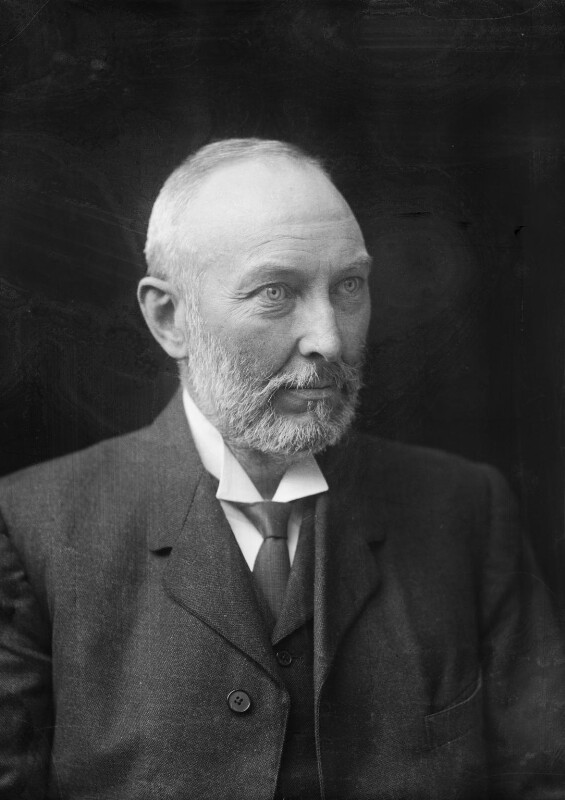
\includegraphics[scale=0.07]{imgs/stoney.jpg}
        \caption{George Gerald Stoney (1863-1942)}
    \end{figure}

    \begin{itemize}
        \item Supposons que $\frac{h_f}{h_s} \ll 1$
        \item Quelle est la courbure $c$ prise par l'ensemble ?
    \end{itemize}
    
    \begin{figure}
        \centering
        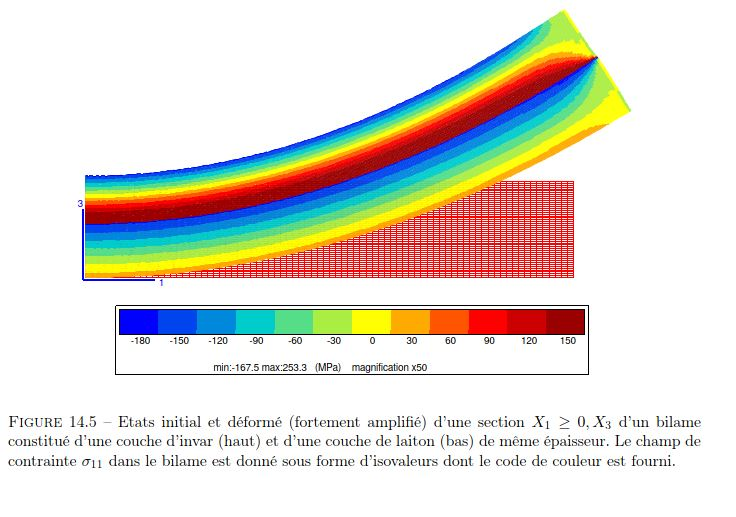
\includegraphics[scale=0.2]{imgs/deformation.JPG}
        \caption{Résultat de simulation}
    \end{figure}
    
\end{frame}


% 1m

\begin{frame}
    \frametitle{La formule de Stoney (1909)}

    \begin{itemize}
        \item $c = 6\frac{M_fh_f}{M_sh_s^2}(\alpha_s-\alpha_f)(T-T_0)$ si $M_fh_f \ll M_sh_s$ 
        \item Dans les autres directions ? Courbure nulle ou parabolique
        \item Permet de prévoir la déformation de l'ensemble, en combinant ls caractéristiques géométriques et les propriétés mécaniques des couches
    \end{itemize}
    
    \begin{figure}
        \centering
        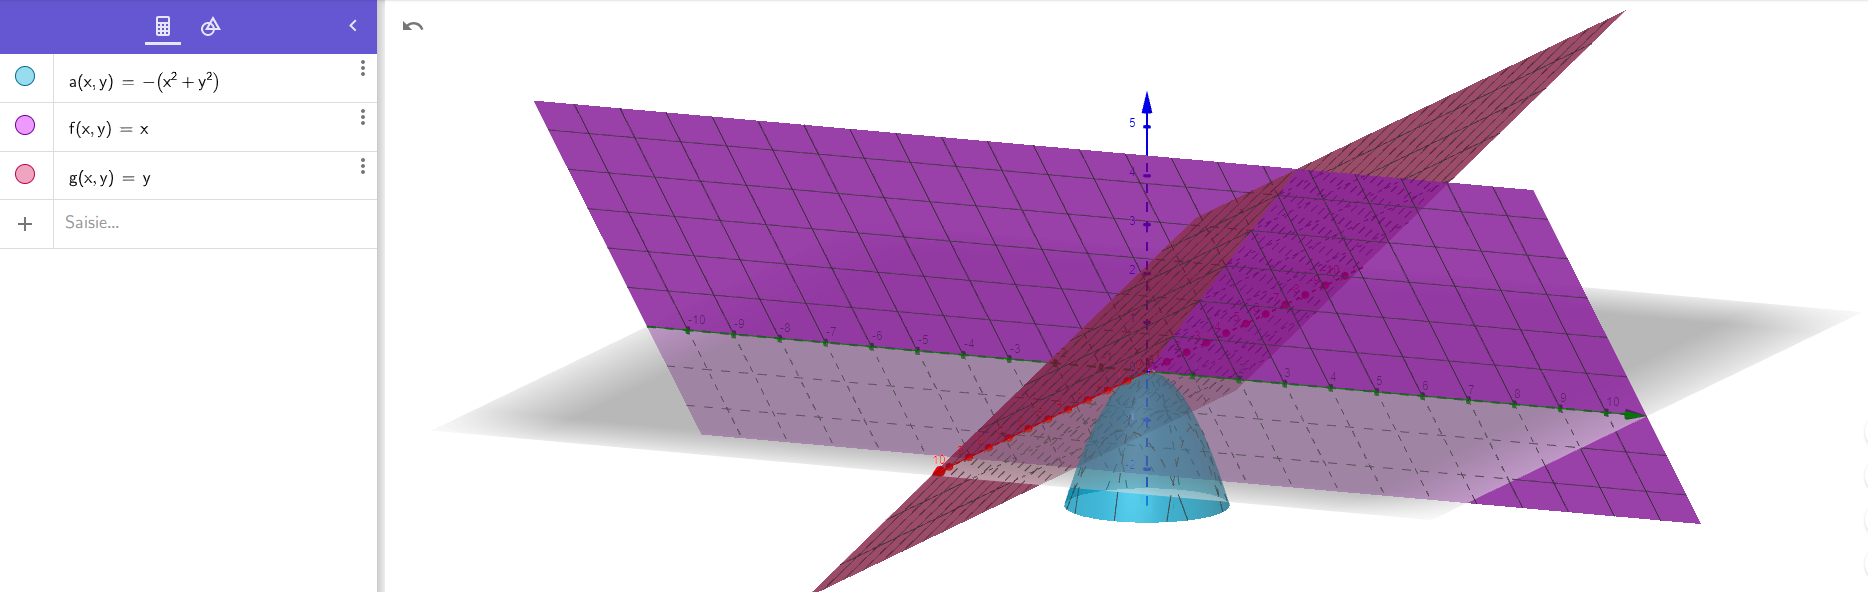
\includegraphics[scale=0.25]{imgs/courbes.png}
        \caption{Paraboloïde de révolution et hyperplans}
    \end{figure}
    
\end{frame}

% 4m15

\begin{frame}
    \frametitle{La formule de Stoney (1909)}

    \begin{itemize}
        \item Qu'évoquait l'article de Stoney ?
        \item Une formule estimant sous certaines conditions (précédemment évoquées) pour déterminer en mesurant la tension et la courbure la couche de nickel déposée sur une électrode 
        \item Reliait la valeur des contraintes à la courbure de l'électrode avec son dépôt
        \item Formule 2D améliorée par Berry en 1988
    \end{itemize}
    
\end{frame}

% 4m45

\begin{frame}
\frametitle{Expérience sommaire : présentation}
\begin{itemize}
    \item Découper des bandes (8 cm par 1 cm environ)
    \item Feuille d'aluminium : $\alpha_f = 23 \times 10^{-6} K^{-1}$, $h_f = 0.02 mm$, $E_f = 62 GPa$, $\nu_f = 0.35$
    \item Papier bristol : $\alpha_s = 3 \times 10^{-6} K^{-1}$, $h_s = 0.3 mm$, $E_s = 3 GPa$, $\nu_s = 0.2$
    \item Colle pour fixer les deux morceaux
    \item Bougie : $T = 200$ °C (juste en-dessous de la température d'auto-inflammation du papier) et $T_0 = 25$ °C
    \item C'est parti !
\end{itemize}
\end{frame}

% 6m

\begin{frame}
\frametitle{Expérience sommaire : résultats}
    \begin{itemize}
        \item Les se dilatent différemment sous l'effet de la chaleur
        \item On remarque que c'est l'aluminium qui est sur la face externe de la courbure. 
        \item On est bien dans le cas des petites déformations avec $||Grad(\underline{u})|| \ll 1$.
        \item On peut chercher à vérifier le signe de la courbure dans la formule de Stoney, même si la deuxième hypothèse $M_f h_f << M_s h_s$ n'est pas vraiment vérifiée :
        \begin{itemize}    
            \item $T-T_0 > 0$
            \item $\alpha_s - \alpha_f < 0$
            \item Donc $c < 0$ (la courbure est vers le bas)
        \end{itemize}
        \item Diversité des applications de cet effet (ici, Stoney, électronique)
    \end{itemize}
\end{frame}

%6m30


\subsection{Contraintes dans un film mince sur un substrat} % A subsection can be created just before a set of slides with a common theme to further break down your presentation into chunks

\begin{frame}
\frametitle{Forme simplifiée des contraintes sous les hypothèses de Stoney}
\begin{itemize}
    \item Contrainte moyenne : $\bar{\sigma}_{11}=\frac{1}{h}\int\sigma_{11}\rm{d}X_3$
    \item Développons au premier ordre $\Delta$, $C$ et $A$
    \item $\sigma_{11}^f=M_f(AX_3+C-\alpha_f(T-T_0)) \approx M_f (\alpha_s - \alpha_f)(T-T_0)$
    \item $\sigma_{11}^s=M_s(AX_3+C-\alpha_s(T-T_0)) \approx \frac{M_fh_f}{M_sh_s} (\alpha_f-\alpha_s)(T-T_0)(6\frac{X_3}{h_s}+4)$
\end{itemize}
\end{frame}

% 8m

\begin{frame}
    \frametitle{Forme simplifiée des contraintes sous les hypothèses de Stoney}
    \begin{itemize}
        \item Par équi-biaxialité, $\bar{\sigma}_{11}^f=\bar{\sigma}_{22}^f=M_f(\alpha_s-\alpha_f)(T-T_0)$, ce qui est un résultat remarquable (ne dépend pas de la géométrie ni des propriétés élastiques du substrat, que de propriétés thermoélastiques du film et du désaccord de dilatation)
        \item De même, $\bar{\sigma}_{11}^s=\bar{\sigma}_{22}^s=M_f\frac{h_f}{h_s}(\alpha_f-\alpha_s)(T-T_0)$
        \item La contrainte moyenne est donc nulle (cohérent car il n'y a pas de chargement extérieur et l'on est en statique, que des contraintes locales à l'intérieur)
        \item Quelle est la fibre neutre ?
    \end{itemize}
\end{frame}

% 9m15

\begin{frame}
    \frametitle{Fibre neutre}
    \begin{itemize}
        \item $\sigma_{11}^s=0 \implies X_3 \simeq \frac{-2h_s}{3}$ (cohérent, bien dans le substrat, car contrainte constante dans le film)
        \item Confirmation par représentation graphique et l'article de Stoney (pas le cas pour l'exemple de la partie précédente)
    \end{itemize}
\end{frame}

% 10m